% Feature Importance Analysis Section
% To be integrated into main.tex

\subsection{Feature Importance Analysis}

To understand the mechanism underlying catastrophic failures, we conducted SHAP~\citep{lundberg2017unified} feature importance analysis on two contrasting tasks: \texttt{sales-shipcond} (catastrophic, 71.6\% coverage drop) and \texttt{sales-office} (robust, 0.1\% drop). We hypothesized that catastrophic tasks would rely on features with low temporal stability, measured by Jaccard similarity between training and test feature value sets.

\textbf{Surprising finding:} Both tasks exhibited \emph{complete feature distribution shift} with 0\% Jaccard similarity across all features, yet their coverage drops differed by 700×. This rules out feature value overlap as the primary mechanism and points to a more subtle phenomenon: \emph{feature importance dynamics under distribution shift}.

Figure~\ref{fig:shap} reveals the key distinction. In the catastrophic task (Panel A), the dominant feature \texttt{SALESDOCUMENT} experiences a concentrated importance explosion from 1.98 to 9.00 (4.5× increase) while maintaining its top ranking. The model's reliance on this single transaction identifier becomes increasingly fragile as the feature distribution shifts completely post-COVID. In contrast, the robust task (Panel B) exhibits dramatic importance redistribution: the top-ranked feature changes from \texttt{SALESDOCUMENT} (1.10) to \texttt{BILLINGCOMPANYCODE} (11.46), with multiple features experiencing 10-20× increases.

Panel C quantifies this difference in importance dynamics. The catastrophic task shows a concentrated 4.5× increase in its top feature, followed by moderate increases (2-4×) in secondary features. The robust task distributes larger increases (7-23×) across all top-5 features, preventing single-feature dependence. Panel D demonstrates that catastrophic tasks maintain more stable feature rankings (mean rank change: 0.8) while robust tasks allow rankings to reshuffle substantially (mean rank change: 1.6), enabling the model to adapt to new data patterns.

\textbf{Mechanism insight:} Catastrophic failure occurs when models develop \emph{single-feature dependence} that breaks under distribution shift. Even with complete feature value turnover, models remain robust if they can \emph{redistribute importance across multiple features}. This suggests that conformal prediction sets, calibrated on validation data where a single feature dominates, become unreliable when that feature's relationship with the target changes post-shift, even if the feature itself remains available.

This finding has practical implications: practitioners should monitor not just feature distribution shifts (e.g., via Jaccard similarity) but also \emph{feature importance concentration}. Tasks where a single feature accounts for $>$40\% of total SHAP importance may be vulnerable to catastrophic failures under distribution shift, regardless of feature stability.

\begin{figure}[t]
\centering
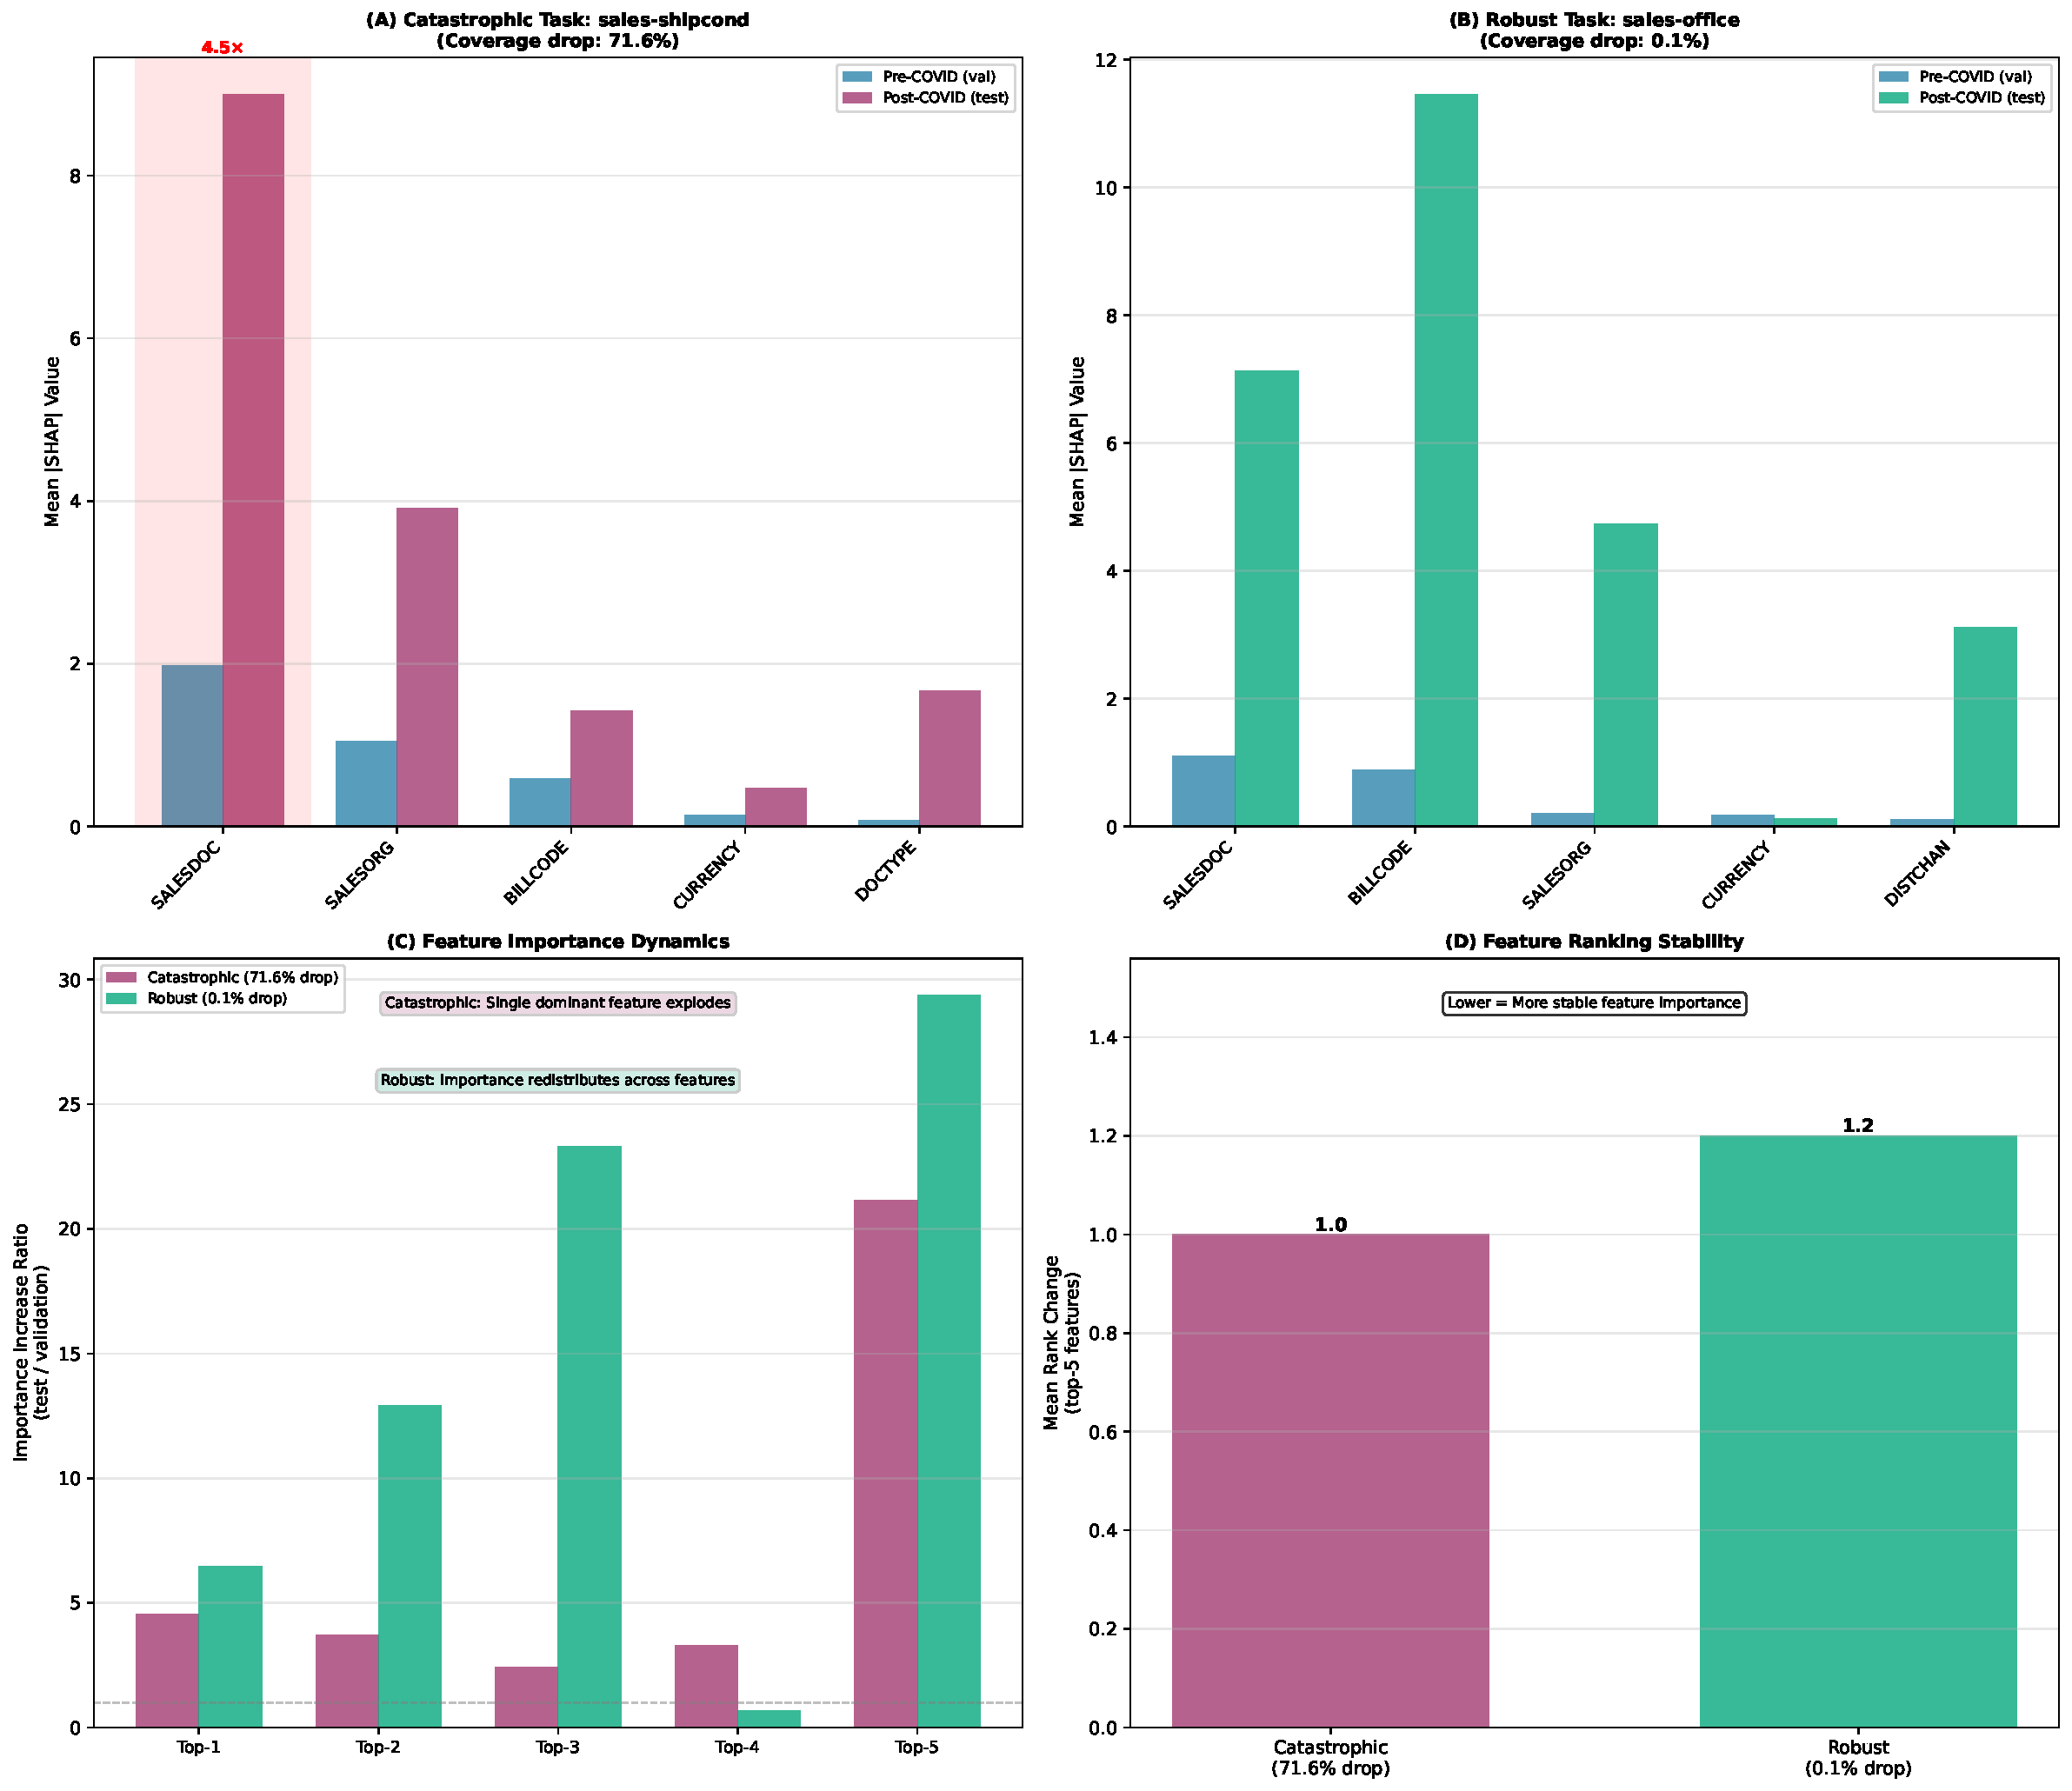
\includegraphics[width=\textwidth]{figures/figure3_feature_importance.pdf}
\caption{\textbf{Feature Importance Analysis reveals mechanism of catastrophic failure.} (A) Catastrophic task: dominant feature \texttt{SALESDOCUMENT} explodes 4.5× while maintaining top rank. (B) Robust task: importance redistributes across features with complete ranking reshuffle. (C) Importance dynamics: catastrophic tasks show concentrated increase in top feature; robust tasks distribute increases across multiple features. (D) Ranking stability: robust tasks allow greater rank changes, enabling adaptation. Despite identical 0\% Jaccard similarity, coverage drops differ by 700× due to feature importance dynamics.}
\label{fig:shap}
\end{figure}
